\documentclass{template}
\begin{document}
%-----请编辑课程--------
\course{某课程}%课程名
%-----请编辑信息--------
\studentname{张三}
\studentclass{究物理01}
\studentid{31415926}
\season{Autumn}
\years{2025}
%---------------------
\maketitle
\newpage
\thispagestyle{empty}
\null
\newpage 
\addtocounter{page}{-2}
\pagenumbering{Roman}
\tableofcontents
\newpage
\thispagestyle{empty}
\null
\newpage 
\pagenumbering{arabic}
\chapter{文档特性}
\newpage
\assignment{文档标题格式}
\subsection{作业集}
调用$\backslash chapter$命令,可以生成大章标题,它被命名为“作业集”,以汉字数字作为序号。
\subsection{作业}
可以调用$\backslash assignment$命令生成作业文档的标题,它相当于$\backslash section$.

然而,为了方便逐次作业提交,这一级别的标题下还缀有个人信息栏。如你所见,信息栏中包含姓名、班级和学号,可以在文首编辑,通用于整个文档中所有的作业。此外,文首还可以编辑课程信息和季节、年份信息。
\begin{lstlisting}[title=\ ,frame=single]
  %个人信息设置
\newcommand{\studentname}[1]{\def\@studentname{#1}}    % 姓名
\newcommand{\studentclass}[1]{\def\@studentclass{#1}} % 班级
\newcommand{\studentid}[1]{\def\@studentid{#1}}  %学号
  %----------
\newcommand{\course}[1]{\def\@course{#1}}  %课程
\newcommand{\season}[1]{\def\@season{#1}}  %季节
\newcommand{\years}[1]{\def\@years{#1}}  %年份
  % 设置编号格式
\counterwithout{section}{chapter}
\renewcommand{\thesection}{作业\chinese{section}}
\titleformat{\section}
  {\centering\zihao{3}\bfseries}
  {\thesection}  % 显示“作业一”
  {1em}
  {}
\end{lstlisting}

同时,新一节的作业会自动转到下一页开始。

另外,你还可以使用$\backslash subsection$命令生成子节,用于标示同一次作业当中不同的部分。
\assignment{习题和解答格式}
可以使用$problem$环境书写题目,并使用$solution$环境进入解答格式。
\begin{problem}
    这是一道习题!
\end{problem}

\begin{solution}
    依旧代码格式:
    \begin{lstlisting}[title=\ ,frame=single]
  %problem
\newcounter{problem}[subsection]
\renewcommand{\theproblem}{\arabic{problem}}

\newmdenv[
  backgroundcolor=gray!10, 
  linewidth=0pt,
  skipabove=12pt,
  skipbelow=12pt, 
  innertopmargin=10pt,
  innerbottommargin=10pt,
  innerleftmargin=15pt,
  innerrightmargin=15pt,
  roundcorner=0pt
]{problembox} 


\newenvironment{problem}[1][]{
  \stepcounter{problem}
  \begin{problembox}
  \textbf{习题 \theproblem \ \ \kaishu}
  \ifx\\#1\\\relax\else\quad (#1)\fi
}{
  \end{problembox}
}

  %solution
\newtheorem*{solution}{\heiti 解}
    \end{lstlisting}
\end{solution}

如你所见,在解答格式当中,字体被设置为$\backslash kaishu$楷体。

另外,习题编号是绑定到$subsection$的。
\assignment{其它特性}
\subsection{作业独立编号}
作业的编号与作业集无关,因此你可以根据需要划分作业集而不用担心影响作业的序号。
\subsection{页码}
本文档在目录处采用大写阿拉伯数字作页码,在正文部分则采用阿拉伯数字页码,正文页码从第一个$chapter$所处页开始计数。
\subsection{d'Alembert算符}
本文档还特别含有了d'Alembert算符,它的数学定义为
\[\dalembert=\frac{1}{c^2}\frac{\partial^2}{\partial t^2}-\nabla^2\]

如今,你可以使用$\backslash dalembert$命令来调用它。
\chapter{示例}
\assignment{Maxwell方程组}
\begin{mdframed}
  \centering
    本节是一般格式的示例
\end{mdframed}
\begin{problem}
    分析一块正在充电的圆形(半径为$R$)平行板电容器周围的磁场分布。
\end{problem}
\begin{solution}
    由
    \begin{equation}
        \oint\mathbf{B}\cdot d\mathbf{l}=\mu_0 \varepsilon_0\frac{d\Phi_E}{dt}
    \end{equation}
    
    得
    \begin{equation}
        B\cdot2\pi R=\mu_0\varepsilon_0\pi R^2\frac{dE}{dt}
    \end{equation}
    
    故
    \begin{equation}
        B=\frac{1}{2}\mu_0\varepsilon_0R\frac{dE}{dt}
    \end{equation}
\end{solution}

\begin{problem}
    如果磁单极存在,如何改写真空中的Maxwell方程组?
\end{problem}
\begin{solution}
    \begin{subequations}
    \begin{equation}
        \nabla\cdot\mathbf{E}=\frac{\rho}{\varepsilon_0}
    \end{equation}
    \begin{equation}
        \nabla\cdot\mathbf{B}=\mu_0\rho_m
    \end{equation}
    \begin{equation}
        \nabla\times\mathbf{E}=-\mu_0\mathbf{J_m}-\frac{\partial\mathbf{B}}{\partial t}
    \end{equation}
    \begin{equation}
        \nabla\times\mathbf{B}=\mu_0\mathbf{J}+\mu_0\varepsilon_0\frac{\partial\mathbf{E}}{\partial t}
    \end{equation}
    \end{subequations}
\end{solution}
\begin{problem}
    由真空中的Maxwell方程组推导电荷守恒定律。
\end{problem}
\begin{solution}
    由
    \begin{equation}
        \nabla\times\mathbf{B}=\mu_0\mathbf{J}+\mu_0\varepsilon_0\frac{\partial\mathbf{E}}{\partial t}
    \end{equation}
    
    得
    \begin{equation}
        0=\mu_0\nabla\cdot\mathbf{J}+\mu_0\varepsilon_0\nabla\cdot(\frac{\partial\mathbf{E}}{\partial t})
    \end{equation}
    
    又
    \begin{equation}
        \nabla\cdot\mathbf{E}=\frac{\rho}{\varepsilon_0}
    \end{equation}

    故
    \begin{equation}
        \nabla\cdot\mathbf{J}+\frac{\partial \rho}{\partial t}=0
    \end{equation}

    得证。
\end{solution}
\begin{problem}
    由真空中的Maxwell方程组研究电磁场运动方程的波动性。
\end{problem}
\begin{solution}
    对于电场,由
    \begin{equation}
        \nabla\times\mathbf{E}=-\frac{\partial\mathbf{B}}{\partial t}
    \end{equation}
    
    得
    \begin{equation}
        \nabla\times\nabla\times\mathbf{E}=-\frac{\partial(\nabla\times\mathbf{B})}{\partial t}
    \end{equation}

    考虑到
    \begin{equation}
        \nabla\times(\nabla\times\mathbf{E})=\nabla(\nabla\cdot\mathbf{E})-\nabla^2\mathbf{E}
    \end{equation}

    有
    \begin{equation}
        \nabla(\frac{\rho}{\varepsilon_0})-\nabla^2\mathbf{E}=-\frac{\partial(\mu_0 \mathbf{J}+\mu_0\varepsilon_0\frac{\partial\mathbf{E}}{\partial t})}{\partial t}
    \end{equation}

    即
    \begin{equation}
        \nabla^2\mathbf{E}-\mu_0\varepsilon_0\frac{\partial^2\mathbf{E}}{\partial t^2}=\nabla(\frac{\rho}{\varepsilon_0})+\mu_0\frac{\partial\mathbf{J}}{\partial t}
    \end{equation}

    对于行进的电磁波,如光,取$\rho=0,\ \mathbf{J}=0$,故

    \begin{equation}
        \nabla^2\mathbf{E}-\mu_0\varepsilon_0\frac{\partial^2\mathbf{E}}{\partial t^2}=0
    \end{equation}

    正是波动方程。磁场同理,有
    \begin{equation}
        \nabla^2\mathbf{B}-\mu_0\varepsilon_0\frac{\partial^2\mathbf{B}}{\partial t^2}=0
    \end{equation}
\end{solution}
\assignment{应用Maxwell方程组}
\begin{mdframed}
  \centering
    本节是带有子节的格式的示例
\end{mdframed}
\subsection{电磁场用势函数表示}
\begin{problem}
    试证明:一定可以找到一组满足洛伦兹规范条件的$\vec{A}$和$\varphi$,并且即使满足洛伦兹规范条件,$\vec{A}$和$\varphi$仍不是唯一的。
\end{problem}
\begin{solution}
原势
\begin{equation}
\varphi(\vec r,t),\quad \vec A(\vec r,t),
\end{equation}

做规范变换
\begin{equation}
\begin{cases}
\varphi' = \varphi - \displaystyle\frac{\partial\lambda}{\partial t},\\
\vec A' = \vec A + \nabla\lambda
\end{cases}
\end{equation}

洛仑兹规范条件
\begin{equation}
\frac{1}{c^2}\frac{\partial\varphi'}{\partial t} + \nabla\!\cdot\!\vec A' = 0
\end{equation}

代入上式可得
\begin{equation}
\frac{1}{c^2}\frac{\partial\varphi}{\partial t}
+ \nabla\!\cdot\!\vec A
+ \Bigl(\frac{1}{c^2}\partial_t^2 - \nabla^2\Bigr)\lambda
= 0
\quad\Longrightarrow\quad
\nabla^2\lambda-\frac{1}{c^2}\frac{\partial^2\lambda}{\partial t^2} = -\Bigl(\frac{1}{c^2}\frac{\partial \varphi}{\partial t} + \nabla\!\cdot\!\vec A\Bigr),
\end{equation}

如令
\begin{equation}
f=(\frac{1}{c^2}\frac{\partial \varphi}{\partial t} + \nabla\!\cdot\!\vec A)
\end{equation}

则构成一个d'Alembert方程,总是有解。因此总能找到一个$\varphi$对应一组$\vec{A}$和$\varphi$,满足洛伦兹规范。


若再对已满足洛仑兹规范的势做一次规范变换,有如(4.2),则
\begin{equation}
    \nabla\cdot\vec{A}+\nabla^2\lambda+\frac{1}{c^2}(\frac{\partial \varphi}{\partial t}-\frac{\partial^2\lambda}{\partial t^2})=0
\end{equation}

考虑到势已经满足洛伦兹变换,故
\begin{equation}
    \nabla^2\lambda-\frac{1}{c^2}\frac{\partial^2\lambda}{\partial t^2} =0
\end{equation}

仍是d'Alembert方程,有非零解。得证。
\end{solution}
\begin{problem}
    在静电、静磁情况下,如何用势函数表示相应的电场和磁场?它们满足的场方程分别是什么?
\end{problem}
\begin{solution}
    \item[\textbf{(1) 静电场}]  
    对于静止电荷分布 \(\rho(\vec r)\),电场 \(\vec E\) 满足
    \begin{equation}
      \nabla \times \vec E = \vec 0,
      \qquad
      \nabla \cdot \vec E = \frac{\rho}{\varepsilon_0}.
    \end{equation}
    由于旋度为零,可引入电势 \(\varphi(\vec r)\),使
    \begin{equation}
      \vec E = -\,\nabla \varphi.
    \end{equation}
    由此,得
    \begin{equation}
      \nabla^2 \varphi = -\,\frac{\rho}{\varepsilon_0}.
    \end{equation}

  \item[\textbf{(2) 静磁场}]  
    对于稳恒电流分布 \(\vec J(\vec r)\),磁场 \(\vec B\) 满足
    \begin{equation}
      \nabla \cdot \vec B = 0,
      \qquad
      \nabla \times \vec B = \mu_0\,\vec J
    \end{equation}
    由于散度为零,可引入矢势 \(\vec A(\vec r)\),使
    \begin{equation}
      \vec B = \nabla \times \vec A 
    \end{equation}
    由此,得
    \begin{equation}
      \nabla \times (\nabla \times \vec A)
      = \mu_0\,\vec J
      \quad\Longrightarrow\quad
      \nabla(\nabla\!\cdot\!\vec A)
      - \nabla^2 \vec A
      = \mu_0\,\vec J 
    \end{equation}
    选取库仑规范
    \(\nabla\!\cdot\!\vec A = 0\),则简化为
    \begin{equation}
      \nabla^2 \vec A = -\,\mu_0\,\vec J 
    \end{equation}
\end{solution}
\subsection{介质中的Maxwell方程组}
\begin{problem}
    由 Maxwell 方程组出发,在均匀介质(电导率 $\sigma$,介电常数 $\varepsilon$)内,求:
\begin{enumerate}
  \item[(1)] 自由电荷体密度 $\rho_f$ 与时间 $t$ 的关系;
  \item[(2)] 极化电荷体密度 $\rho_p$ 与自由电荷体密度 $\rho_f$ 的关系。
\end{enumerate}
\end{problem}
\begin{solution}
\item[\textbf{(1)}] 由于
\begin{equation}
\frac{\partial \rho_f}{\partial t} + \nabla\!\cdot\!\mathbf J_f = 0
\,,\qquad
\mathbf J_f = \sigma\,\mathbf E,
\end{equation}
且在均匀线性介质中,
\begin{equation}
\nabla\!\cdot\!\mathbf E = \frac{\rho_f}{\varepsilon} 
\end{equation}
故
\begin{equation}
\frac{\partial \rho_f}{\partial t}
+ \nabla\!\cdot(\sigma\,\mathbf E)
= \frac{\partial \rho_f}{\partial t}
+ \sigma\,\frac{\rho_f}{\varepsilon}
=0 
\end{equation}
即
\begin{equation}
\rho_f(t)
= \rho_f(0)\,\exp\!\Bigl(-\frac{\sigma}{\varepsilon}\,t\Bigr) 
\end{equation}
\item[\textbf{(2)}] 
\begin{equation}
\rho_p = -\,\nabla\!\cdot\!\mathbf P,
\end{equation}
而
\begin{equation}
\mathbf D = \varepsilon_0\,\mathbf E + \mathbf P
= \varepsilon\,\mathbf E,
\quad
\nabla\!\cdot\!\mathbf D = \rho_f 
\end{equation}
故
\begin{equation}
\mathbf P = (\varepsilon - \varepsilon_0)\,\mathbf E
\quad\Longrightarrow\quad
\rho_p
= -\,(\varepsilon - \varepsilon_0)\,\nabla\!\cdot\!\mathbf E
= -\,(\varepsilon - \varepsilon_0)\,\frac{\rho_f}{\varepsilon}
= -\Bigl(1 - \frac{\varepsilon_0}{\varepsilon}\Bigr)\,\rho_f 
\end{equation}
\end{solution}
\begin{problem}
    电流稳定地流过两个导电介质的交界面,已知介质 1 的电导率和介电常数分别为 \(\sigma_1,\varepsilon_1\),介质 2 的电导率和介电常数分别为 \(\sigma_2,\varepsilon_2\)。交界面处介质 1 和介质 2 的电流密度分别为 \(\mathbf j_1\) 和 \(\mathbf j_2\)。试求交界面上的自由电荷面密度 \(\sigma_f\) 
\end{problem}
\begin{solution}

由边界条件,
\begin{equation}
\sigma_{f}
= D_{1n} - D_{2n}
= \varepsilon_{1}E_{1n} \;-\; \varepsilon_{2}E_{2n} 
\end{equation}

如题,两介质中
\begin{equation}
j_{1} = \sigma_{1}E_{1n},
\qquad
j_{2} = \sigma_{2}E_{2n},
\end{equation}

从而
\begin{equation}
E_{1n} = \frac{j_{1}}{\sigma_{1}},
\qquad
E_{2n} = \frac{j_{2}}{\sigma_{2}} 
\end{equation}

故
\begin{equation}
\sigma_{f}
= \varepsilon_{1}\,\frac{j_{1}}{\sigma_{1}}
  \;-\;
  \varepsilon_{2}\,\frac{j_{2}}{\sigma_{2}} 
\end{equation}
\end{solution}
\begin{problem}
    证明:当两种绝缘介质的界面上不带面自由电荷时,界面上电场线的折射满足
\[
\frac{\tan\theta_2}{\tan\theta_1}=\frac{\varepsilon_2}{\varepsilon_1},
\]
其中 $\varepsilon_1,\varepsilon_2$ 分别为两介质的介电常数,$\theta_1,\theta_2$ 分别为界面两侧电场线与法线的夹角。

\end{problem}
\begin{solution}
    由题,
\begin{equation}
D_{1n}=D_{2n}
\quad\Longrightarrow\quad
\varepsilon_1\,E_{1n}=\varepsilon_2\,E_{2n} 
\end{equation}

而
\begin{equation}
E_{1t}=E_{2t} 
\end{equation}

折射角 $\theta_i$($i=1,2$)满足
\begin{equation}
\tan\theta_i=\frac{E_{it}}{E_{in}} 
\end{equation}

故
\begin{equation}
\frac{\tan\theta_2}{\tan\theta_1}
=\frac{E_{2t}/E_{2n}}{E_{1t}/E_{1n}}
=\frac{E_{1t}}{E_{2t}}\;\frac{E_{1n}}{E_{2n}}
=\frac{\varepsilon_2}{\varepsilon_1},
\end{equation}

得证。
\end{solution}
\assignment{镜像法}
\begin{mdframed}
  \centering
    本节是带有图片的格式的示例
\end{mdframed}
\begin{problem}
    如图所示,一无穷大导体平面上有一半径为a的半球形鼓包,这导体不带电。现将一电荷量为q的点电荷放在鼓包的正上方离球心为$b\ (>a)\ $处,这时导体电势为零。试用镜像法求空间电势。\par
    \centering
        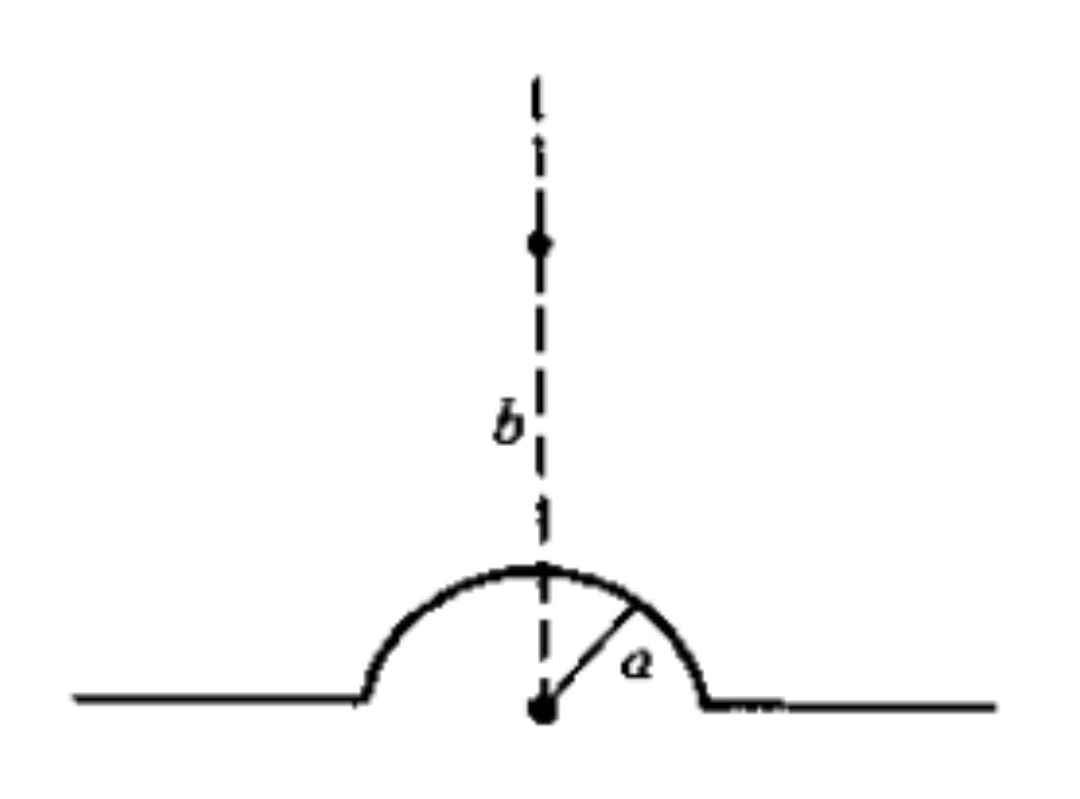
\includegraphics[width=0.2\linewidth]{figures/example1.jpg}
\end{problem}
\begin{solution}
    以球心为坐标原点建立右手系,图中平面取为$yz$平面,$z$轴正方向为竖直向上,则定解条件
    \begin{equation}
        \nabla^2\varphi=-q\delta(x,y,z-b)/\varepsilon_0
    \end{equation}
    
    记空间点与原点的距离为$R$. 考虑到导体表面电势为零,无限远处电势为零,使用镜像法,设置如下像电荷:

    \begin{table}[H]
        \centering
        \begin{tabular}{|c|c|}
            \hline
            位置& 电荷 \\ \hline
            $z=-b$ & $-q$ \\ \hline
            $z=a^2/b$ & $-qa/b$ \\ \hline
            $z=-a^2/b$ & $+qa/b$ \\ \hline
        \end{tabular}
    %\caption{A 2x3 Table Example}
        \label{tab:example_2x3}
    \end{table}
    于是导体外的空间点处电势
    \begin{align}
        \varphi=\frac{1}{4\pi\varepsilon_0}[\frac{q}{\sqrt{x^2+y^2+(z-b)^2}}+\frac{-q}{\sqrt{x^2+y^2+(z+b)^2}}\nonumber\\ +\frac{-qa/b}{\sqrt{x^2+y^2+(z-a^2/b)^2}}+\frac{qa/b}{\sqrt{x^2+y^2+(z+a^2/b)^2}}]
    \end{align}
\end{solution}
\chapter{后记}
\assignment{文档说明}
感谢您使用该模板!欢迎关注我的微信公众号\heiti 我辈都能究物理\songti

\ 

\begin{center}
     
\includegraphics[width=0.9\linewidth]{figures/mychannel.jpg}
\end{center}

如您在使用过程中有意见或建议,敬请通过该公众号与我联系。

祝学业顺利!
\end{document}

